\documentclass[12pt, french]{article}

\usepackage{fancyhdr, fancybox, lastpage}
\usepackage[most]{tcolorbox}
\usepackage[a4paper, margin={0.3in, .75in}]{geometry}
\usepackage{wrapfig}
\pagestyle{fancy}
\renewcommand\headrulewidth{1pt}
\renewcommand\footrulewidth{1pt}
\fancyhf{}
\rhead{ \em{Zakaria Haouzan}}
\lhead[C]{\em{1ére année baccalauréat Sciences Mathématiques}}
\chead[C]{}
\rfoot[C]{}
\lfoot[R]{}
\cfoot[]{\em{Page \thepage / \pageref{LastPage}}}


\newtcolorbox{Box2}[2][]{
                lower separated=false,
                colback=white,
colframe=white!20!black,fonttitle=\bfseries,
colbacktitle=white!30!gray,
coltitle=black,
enhanced,
attach boxed title to top left={yshift=-0.1in,xshift=0.15in},
title=#2,#1}


\begin{document}
\begin{center}
   \shadowbox {\bf{Champ électrostatique}}
\end{center}


%%_________________________Exercice ! :"_________________________Exercice
   \begin{Box2}{Exercice 1 : }
      \begin{wrapfigure}[1]{r}{0.28\textwidth}
  \begin{center}
     \vspace{0.25cm}
    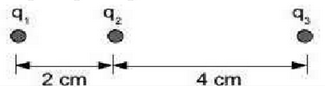
\includegraphics[width=0.28\textwidth]{./img/img_00.png}
  \end{center}
\end{wrapfigure}
      On place trois charges $q_1, q_2$ et $q_3$ comme ci-dessous. 

      Les charges sont telles que $q_1 = q_2 = -q_3$. L'intensité de force exercée par $q_1$ sur $q_2$ est de $3.10^{-2}$N.

1. Déterminer la force que $q_1$ exerce sur $q_3$

2. Déterminer la force résultante des forces exercées sur $q_3$.

On donne $k= 9.10^9$(S.I)
\end{Box2}


%%_________________________Exercice !2 :"_________________________Exercice
\begin{Box2}{Exercice 2 : }
Deux charges électriques +q et –q sont respectivement en A et B telles que AB=2a.

1. Déterminer, en fonction de q, $\varepsilon_0$ et a, les caractéristiques du champ électrostatique au milieu O de AB.

   2. Déterminer l’intensité $E_M$ du champ électrostatique au point M tel que MA=MB=2a.
\end{Box2}

%%_________________________Exercice ! 3:"_________________________Exercice
\begin{Box2}{Exercice 3 :}
Un ensemble de quatre charges électriques ponctuelles +q,-q,+2q et-q placées
respectivement en A, B, C et D sommets d’un carré de côté a = 4 cm.

1. Déterminer les caractéristiques des trois forces électriques s’appliquant sur la charge en A.On donne $q = 10^{-9} C$.

2. Faire une représentation de ces forces à l’échelle.

3. Trouver, graphiquement et par le calcul, la force équivalente appliquée en A. Comparer les valeurs trouvées.
\end{Box2}

%%_________________________Exercice 4 : _________________________Exercice
\begin{Box2}{Exercice 4 : }
On dispose deux plaques métalliques verticalement, l’une en face de l’autre. Elles sont reliées à un générateur de
   manière à ce que le champ électrique entre les deux plaques ait une valeur de E=$2.0 .10^5 V.m^{-1} $ . Les deux plaques sont distantes de d= 20 cm.
Au bout d’un fil, une petite sphère de masse $m = 0.40 g$  entre les deux plaques. Cette sphère est chargée
électriquement, et le fil est incliné d’un angle de $\alpha= 20$° par rapport à la verticale lorsqu’il est soumis au champ
entre les deux plaques. Le fil est incliné vers la plaque chargée négativement.

1. Déterminer le signe de la charge de la sphère.
   
2. Déterminer l’intensité du poids, P, de la sphère (on prendra $g=10 N.kg^{-1}$)

3. La sphère étant en équilibre, représenter sur un schéma l’ensemble des forces qui agissent sur la sphère et en déduire la condition d’équilibre.

4. Déduire la valeur de T (latension du fil) puis celle de F l’intensité de la force électrique.

5. En déduire la charge électrique portée par la sphère.
\end{Box2}
%%_________________________Exercice 5 : _________________________Exercice
\begin{Box2}{Exercice 5 : }
   \begin{wrapfigure}[5]{r}{0.28\textwidth}
     \vspace{-0.75cm}
    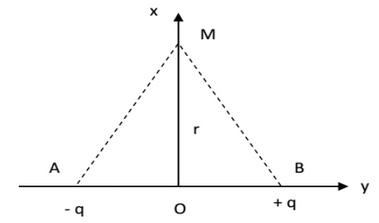
\includegraphics[width=0.28\textwidth]{./img/img_01.png}
\end{wrapfigure}
Soit le dipôle AB, défini dans le repère (O,x,y). Les points A, B et M
ont pour coordonnées : A (-a ;0) et B (a ;0) et A (0 ;r)

1. Donner au point M, les caractéristiques du champ E(A/M) créé par
la charge -q puis celles du champ E(B/M) crée par +q : ( les intensités
seront données en fonction de q, a et r ).

2. Déterminer en fonction de q, r et a les coordonnées du vecteur
champ résultant :

2.1. au point O milieu de [AB].

   2.2. au point de la médiatrice de [AB].

   2.3. Que devient l’intensité du champ en M lorsque OM est très grand devant AB
\end{Box2}


\vspace{2cm}
\begin{center}
   \Large{ \em{Exercices Supplémentaires}}
\end{center}
%%_________________________Exercice 6 : _________________________Exercice
\begin{Box2}{Exercice 6:}
Dans le canon à électrons d’un oscillographe (voir fig.), les électrons sortant de la cathode avec une vitesse
supposée nulle, sont accélérés par une tension U=1600V appliquée entre la cathode C et l’anode A.

1. Calculer en mètres par seconde la vitesse $v_A$ des électrons à la sortie du canon.
   
2. Calculer en joule et en kilo électronvolts, leur énergie cinétique $E_{CA}$
   \begin{center}
    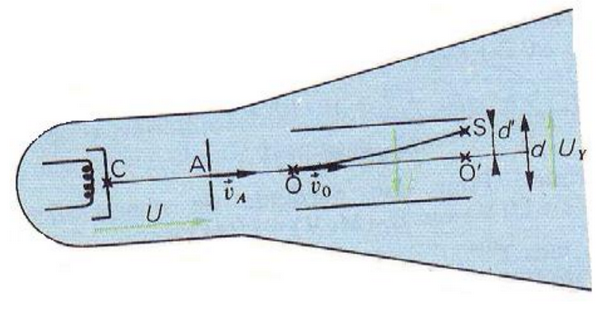
\includegraphics[width=0.5\textwidth]{./img/img_02.png}
      \end{center}
   3. Les électrons pénètrent avec une vitesse $V_O = V_A$, entre les plaques de déviation verticale, en un point O
situé à égale distance de chacune d’elles. Lorsque la tension $U_1 = 500V$ est appliquée à ces plaques
distantes de d = 2cm, les électrons sortent de l’espace champ en un point S tel que O’S=d’=0,6cm.
   \begin{enumerate}
      \item[a.] On prend l’origine des potentiels $V_0$ = 0 au point O. Calculer Vs potentiel électrostatique du point S del’espace champ.

      \item[b.] Déterminer Epo et Eps, énergies potentielles électrostatique d’un électron en O et en S dans l’espace champ, en joules et en kilo électronvolts.

      \item[c.] En déduire $Ec_s$ énergie cinétique de sortie des électrons, en kilo électronvolts.
   \end{enumerate}
\end{Box2}

\begin{Box2}{Exercice 7 :}
  \begin{wrapfigure}{r}{0.28\textwidth}
     \vspace{-0.75cm}
    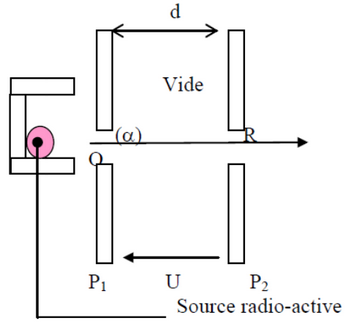
\includegraphics[width=0.28\textwidth]{./img/img_03.png}
\end{wrapfigure}
   Une particule $\alpha$ (noyau d’atome d’hélium), produite par une source radioactive, est mise au voisinage du
point O avec une vitesse négligeable.

   1. Quelle tension $U_{P1P2} = U$ faut-il appliquer entre les plaques $P_1$ et $P_2$,
distantes de $d = 20cm$, pour que la particule traverse la plaque $P_2$ en R, à
la vitesse $v =103km/s$.

2. Donner les caractéristiques du champ électrostatique E (supposé uniforme) entre les plaques.

   3. Quelle est, en joules et en électrons-volts, l’énergie cinétique de la
particule à son passage au point R.
   Données : $m = 6,6.10^{-27}$ kg ; Charge électrique : $q = +2e = +3,2.10^{-19}$ C.
\end{Box2}





\end{document}
